
\documentclass{beamer}
\usepackage[brazil]{babel}
\usepackage[utf8]{inputenc}
\usepackage[T1]{fontenc}
\usepackage{graphicx}
\usetheme{metropolis}           % Use metropolis theme

\title{Uma Abordagem Colaborativa para a Avaliação de Sensores em Ambientes de Internet das Coisas}
\date{\today}
\author{Jônatas Ribeiro Senna Pires}
\institute{Universidade de Brasília}
\begin{document}

  \maketitle

  \begin{frame}{Estrutura da Apresentação}
    \setbeamertemplate{section in toc}[sections numbered]
    \tableofcontents[hideallsubsections]
  \end{frame}

  \section{Contextualização}
    \begin{frame}{Sobre o Trabalho}
      Um sistema colaborativo para avaliação \cite{collaborative} da qualidade dos sensores em um ambiente Internet das Coisas.
    \end{frame}

  \section{Objetivos}
    \begin{frame}{Objetivo Geral}
          \begin{itemize}
            \item Desenvolver o sistema SenseHera, um sistema colaborativo para avaliação de sensores em ambiente IoT, levando em consideração os dados coletados e as informações fornecidas pelos usuários.
          \end{itemize}
    \end{frame}

    \begin{frame}{Objetivos Específicos}
      \begin{itemize}
          \item Desenvolver um ambiente IoT em escala reduzida para teste de conceito;
          \item Desenvolver o SenseHera;
          \item Desenvolver um módulo que realize a avaliação da qualidade dos sensores utilizando:
            \begin{itemize}
              \item Os dados coletados pelos sensores
              \item As informações fornecidas pelos usuários
            \end{itemize}
      \end{itemize}
    \end{frame}

  \section{Sistema SenseHera}
  \begin{frame}{Visão Geral}
    O SenseHera é um sistema web com as funcionalidades para:
    \begin{itemize}
      \item Gestão dos dados produzidos pelos sensores conectados ao ambiente IoT;
      \item Intermediar os usuários e os dados coletados;
      \item Permitir a colaboração por parte dos usuários;
      \item Calcular uma pontuação de qualidade para cada sensor.
    \end{itemize}
  \end{frame}

  \begin{frame}{Requisitos}
    \begin{itemize}
      \item Funcionar em ambientes de baixa capacidade computacional;
      \item Armazenar informações coletadas por sensores;
      \item Apresentar as informações dos sensores de forma simplificada ao usuário;
      \item Escalabilidade e facilidade para adição de sensores;
      \item Permitir o envio de informações sobre fatos e sensações do ambiente pelo usuário;
      \item Baseado nos dados coletados pelos sensores e informações enviadas pelos usuários, calcular uma nota para os dispositivos sensitivos.
    \end{itemize}
  \end{frame}

  \begin{frame}{Funcionamento}
    Idealização das interações
    \begin{center}
    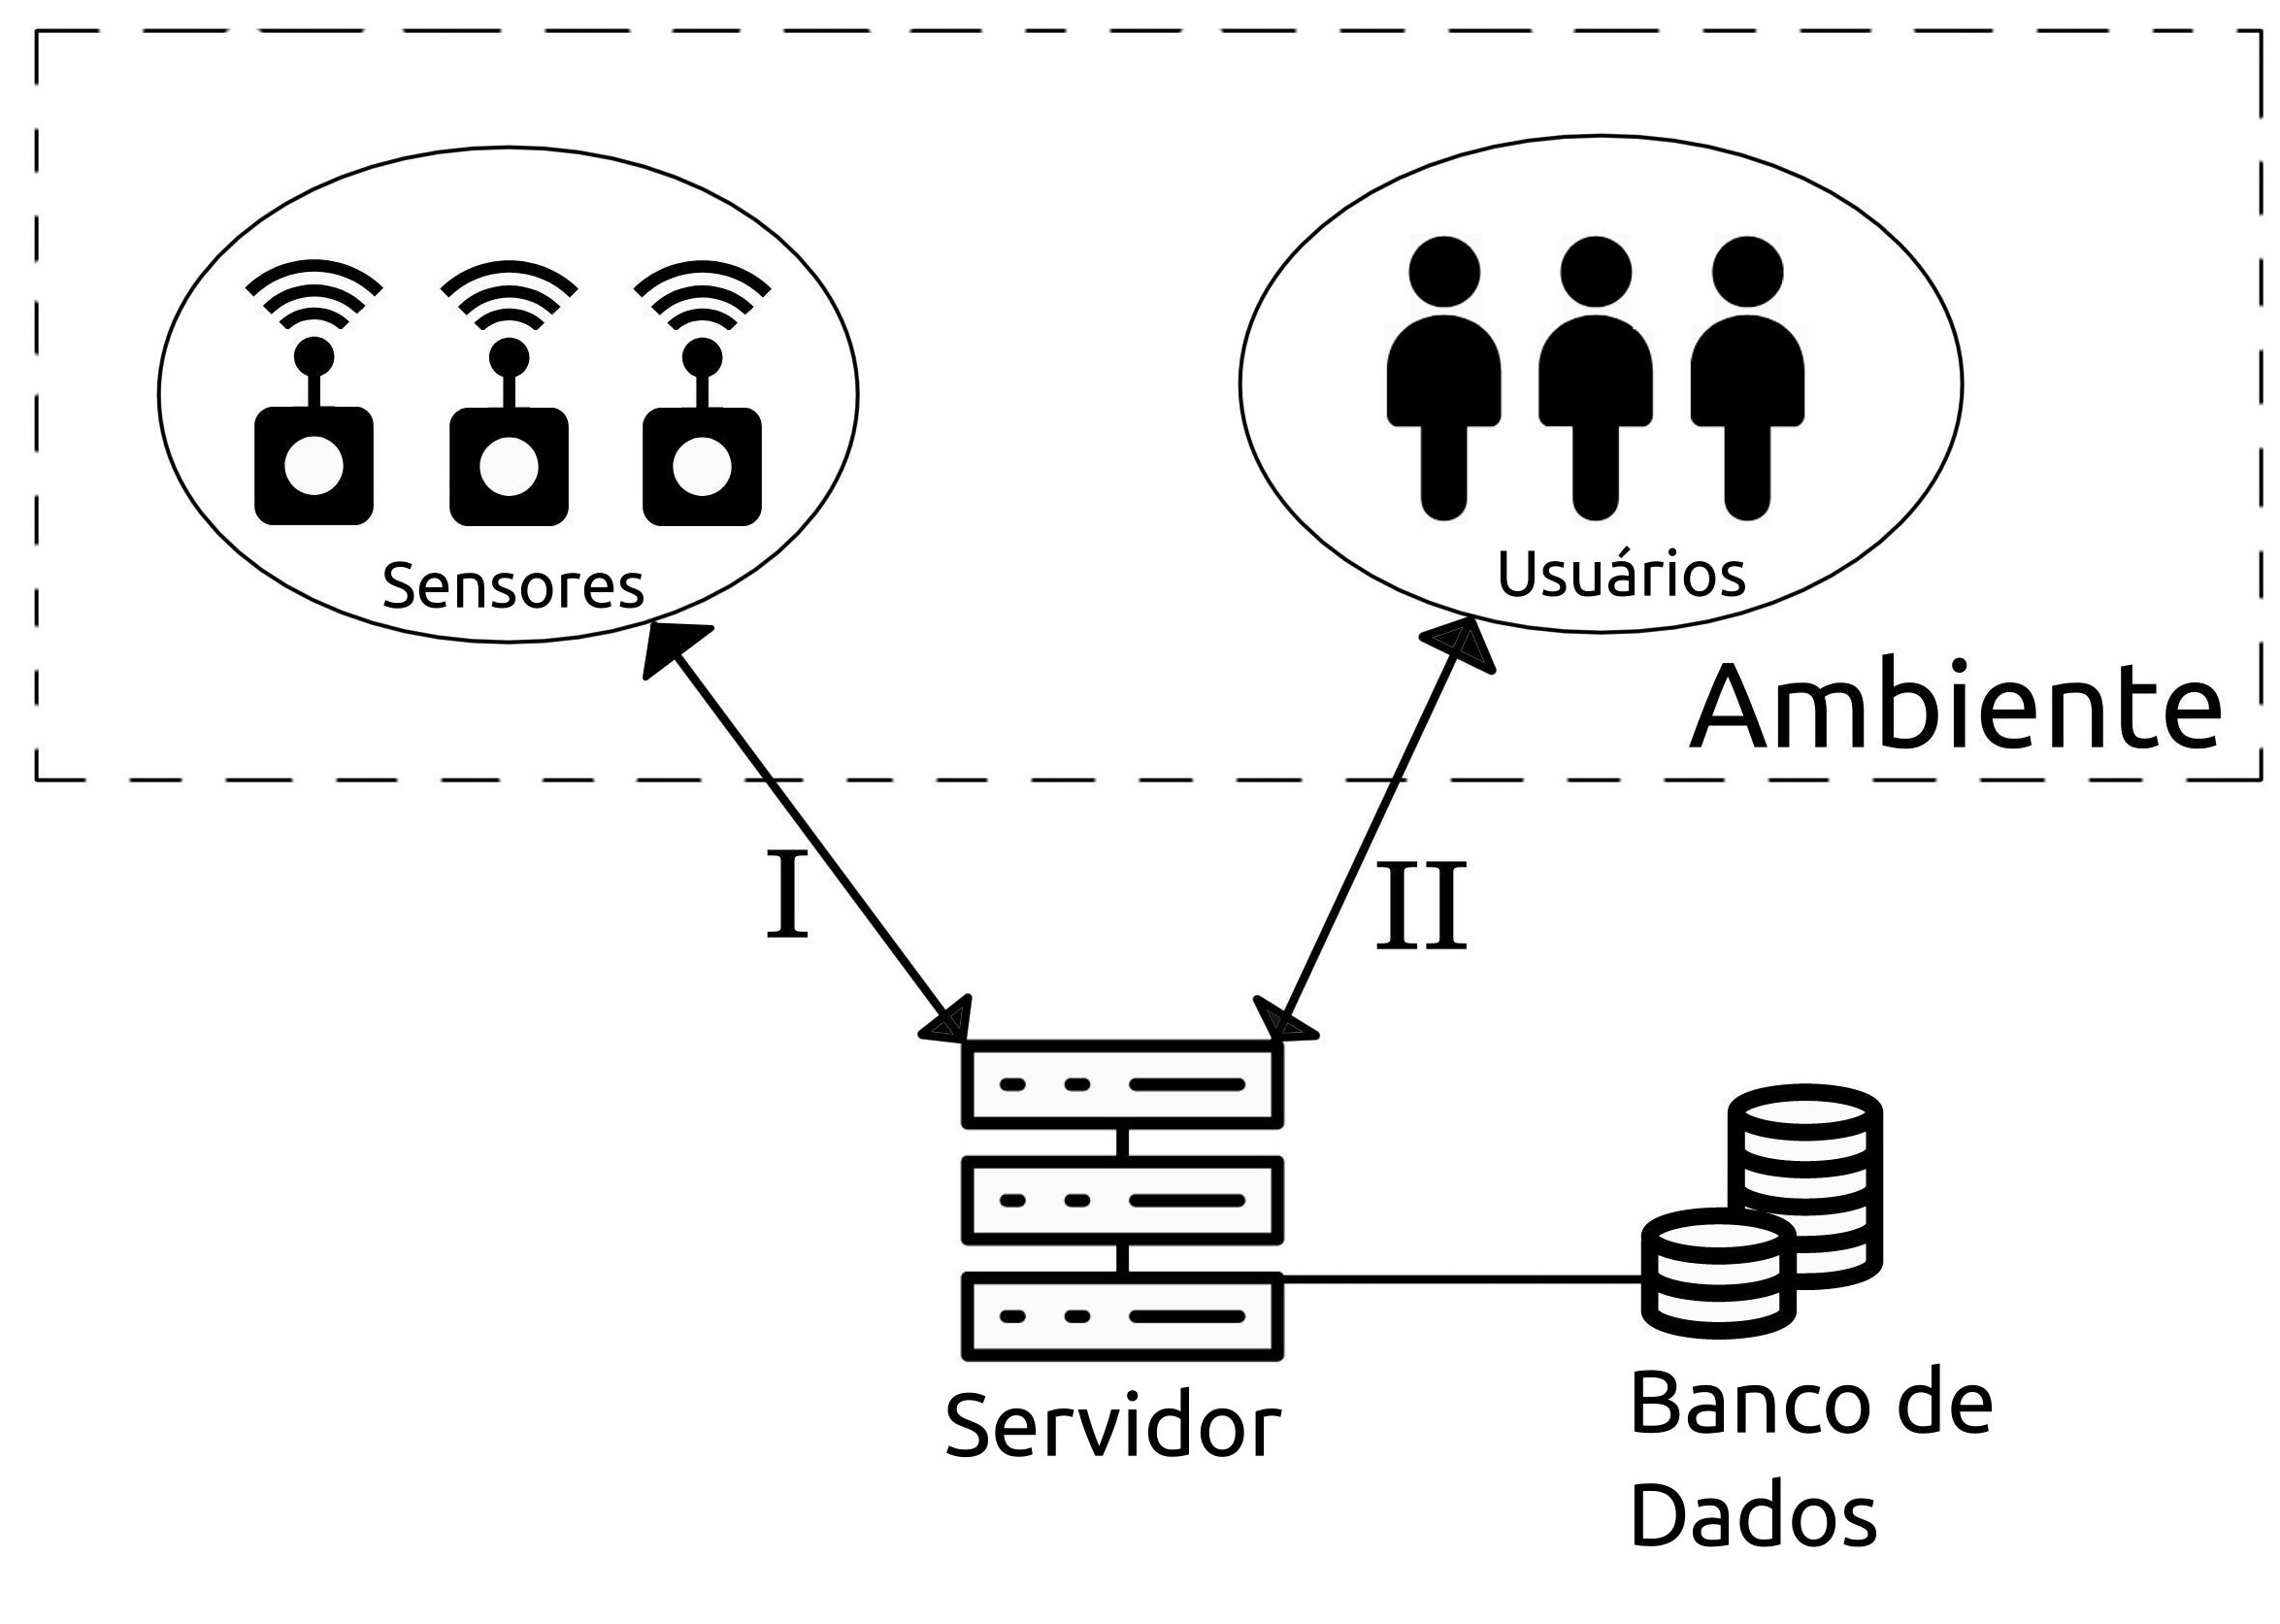
\includegraphics[scale=0.7]{solucao1}
    \end{center}
  \end{frame}
  \begin{frame}{Funcionamento}
    Idealização da colaboração
    \begin{center}
    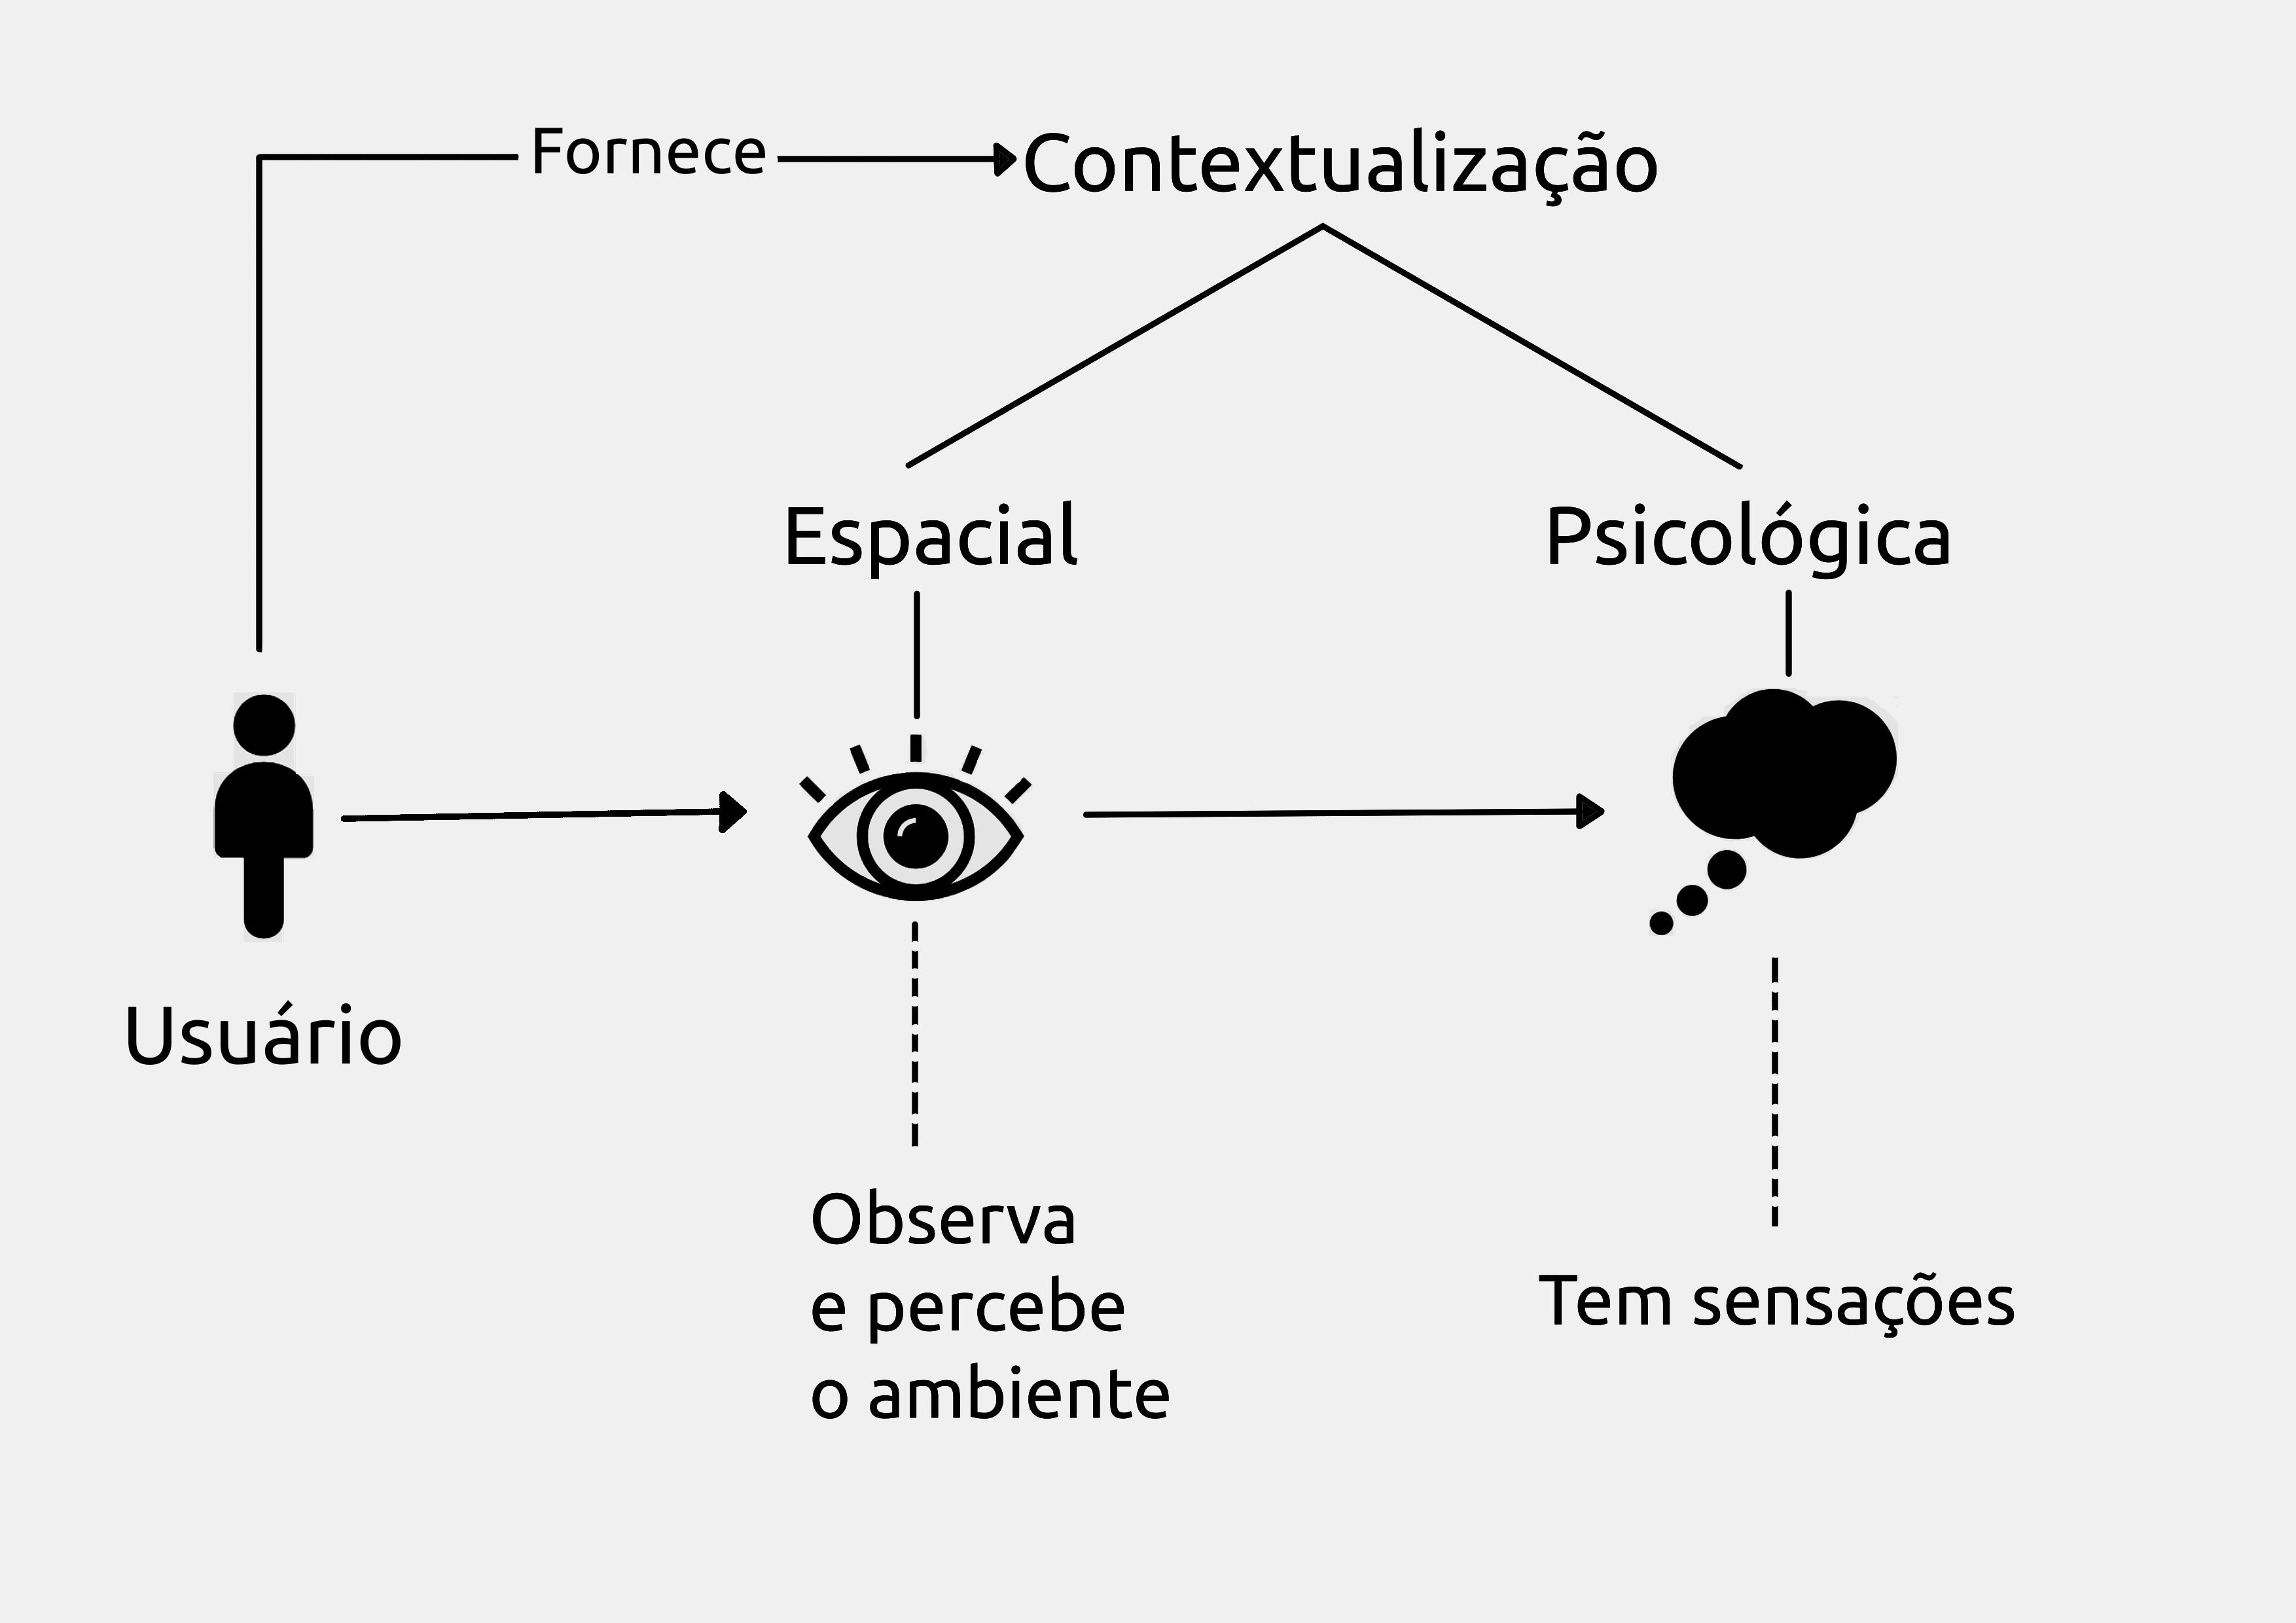
\includegraphics[scale=0.7]{solucao2}
    \end{center}
  \end{frame}

  \begin{frame}{Servidor}
    Foi contratado um serviço online (Amazon Lightsail \cite{lightsail}) para hospedar o sistema, o qual possui as seguintes características:
    \begin{itemize}
      \item Processador de um núcleo;
      \item 512 MB de memória RAM;
      \item 20 GB de SSD para armazenamento.
    \end{itemize}
  \end{frame}
  \begin{frame}{Servidor}
    Neste servidor foram instaladas as seguintes ferramentas:
    \begin{itemize}
      \item SO Ubuntu 18.04;
      \item Python 2.7;
      \item Framework Django;
      \item SGBD PostgreSQL;
      \item Servidor HTTP Apache;
      \item Git.
    \end{itemize}
  \end{frame}

  \begin{frame}{Banco de Dados}
    Diagrama Entidade Relacionamento do sistema
    \begin{center}
    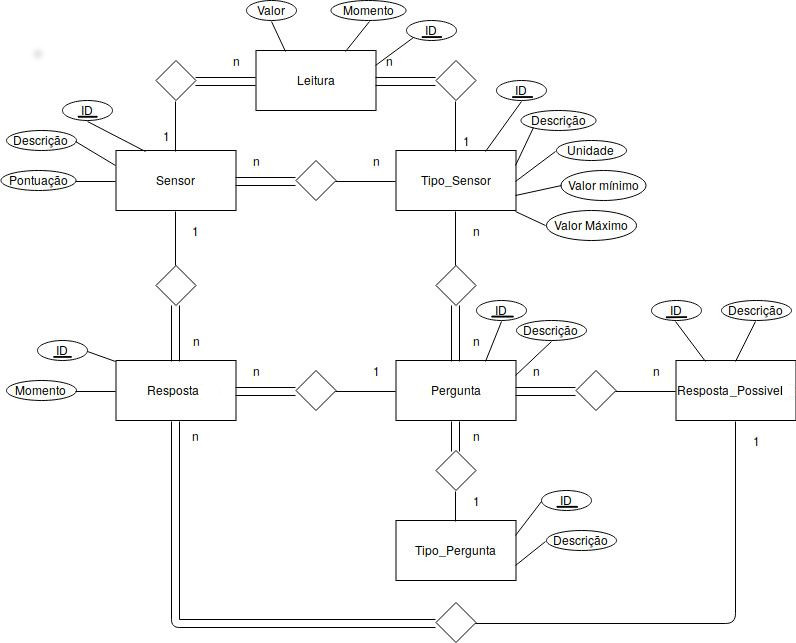
\includegraphics[scale=0.3]{tccDER}
    \end{center}
  \end{frame}

  \begin{frame}{Sistema de Pontuação}

  \end{frame}

  \begin{frame}{Interface do Sistema - Página Inicial}
    Página inicial do sistema
    \begin{center}
    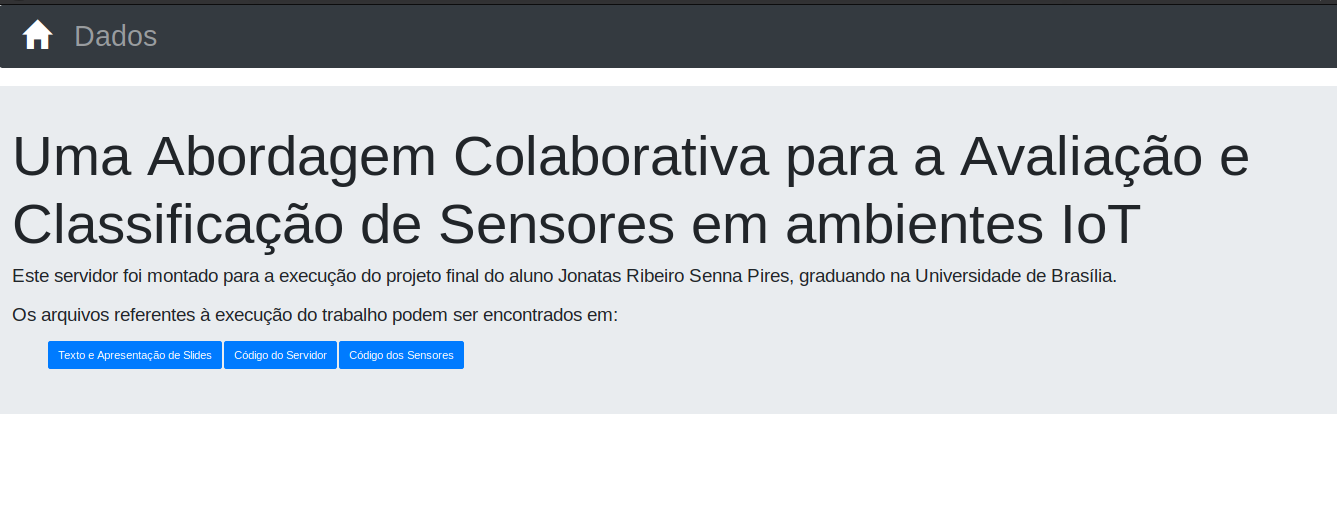
\includegraphics[height=160pt, width=\textwidth]{inicial}
    \end{center}
  \end{frame}
  \begin{frame}{Interface do Sistema - Página Principal}
    Página principal do sistema
    \begin{center}
    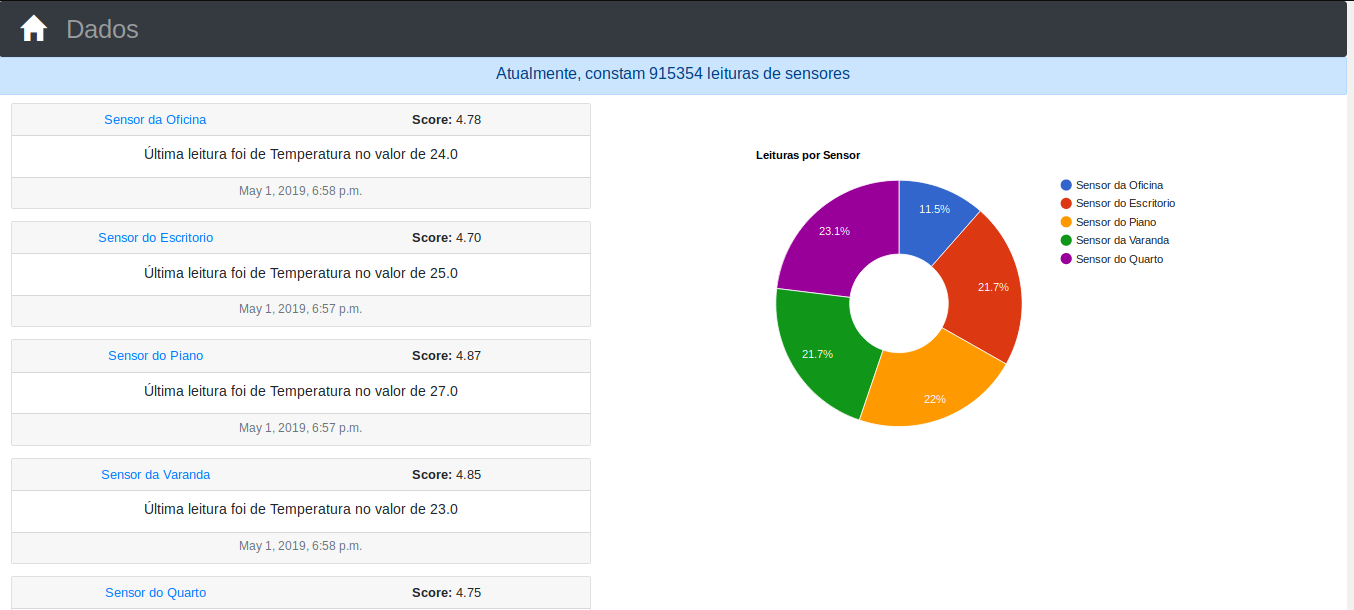
\includegraphics[height=160pt, width=\textwidth]{principal}
    \end{center}
  \end{frame}
  \begin{frame}{Interface do Sistema - Página de Detalhes de um Sensor}
    Página de detalhes de um sensor
    \begin{center}
    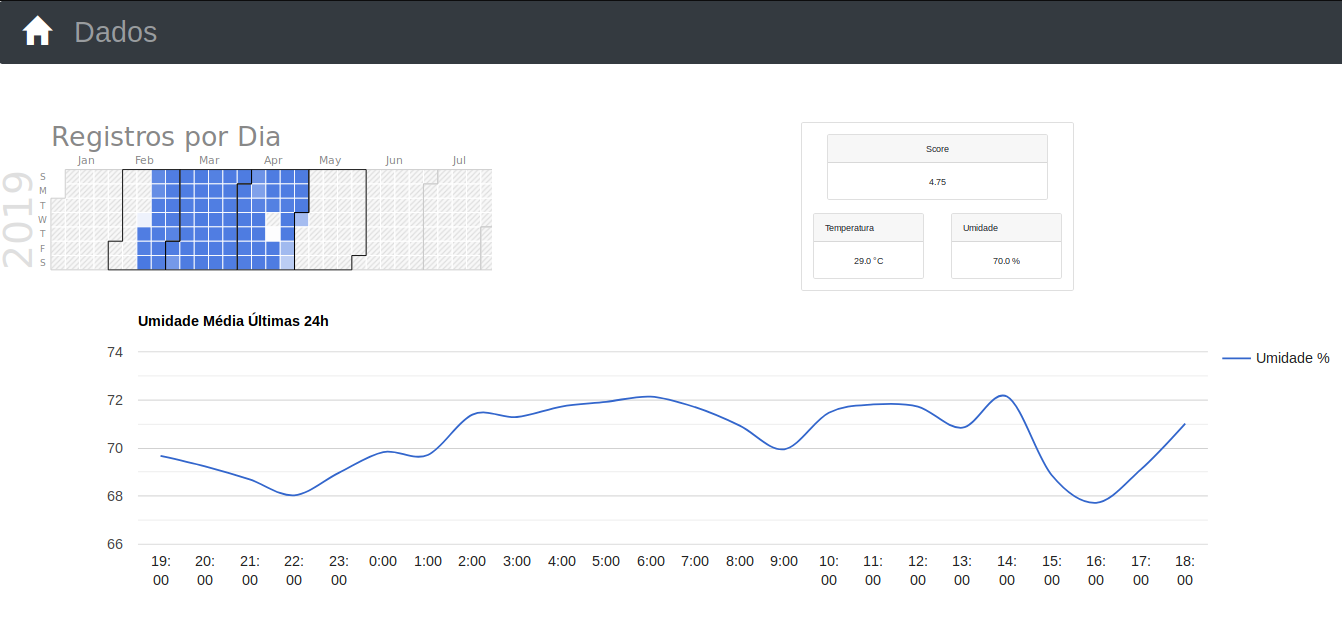
\includegraphics[height=160pt, width=\textwidth]{pSensor}
    \end{center}
  \end{frame}
  \begin{frame}{Interface do Sistema - Página de administração}
    Página de administração
    \begin{center}
    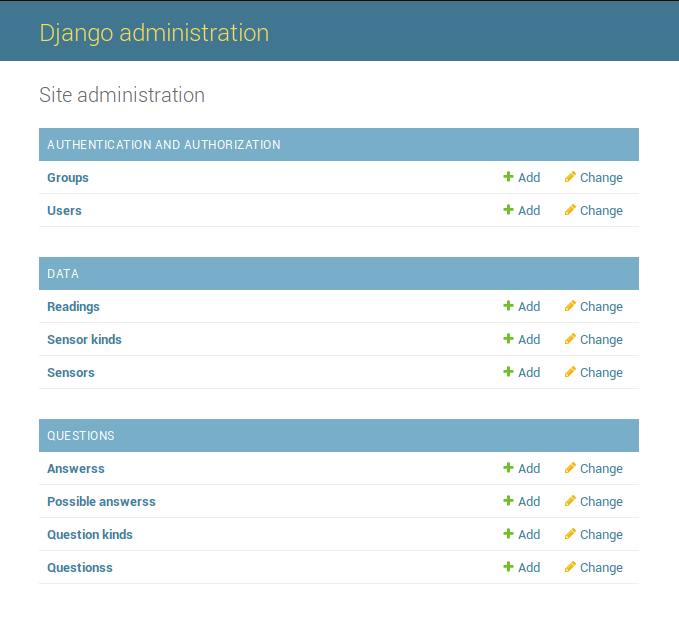
\includegraphics[scale=0.3]{admin}
    \end{center}
  \end{frame}

  \section{Construção do Ambiente IoT em Escala Reduzida}
    \begin{frame}{Visão Geral}
      \quad Foram construídos cinco dispositivos sensitivos para a construção do ambiente IoT em escala reduzida.
      \\\null \quad A construção foi necessária para possibilitar o teste de todas as funcionalidades do sistema.
    \end{frame}

    \begin{frame}{Montagem dos Dispositivos Sensitivos}
      Foram utilizados os seguintes componentes:
      \begin{itemize}
        \item Raspberry Pi Zero W;
        \item Sensor DHT 11;
      \end{itemize}
      \begin{center}
      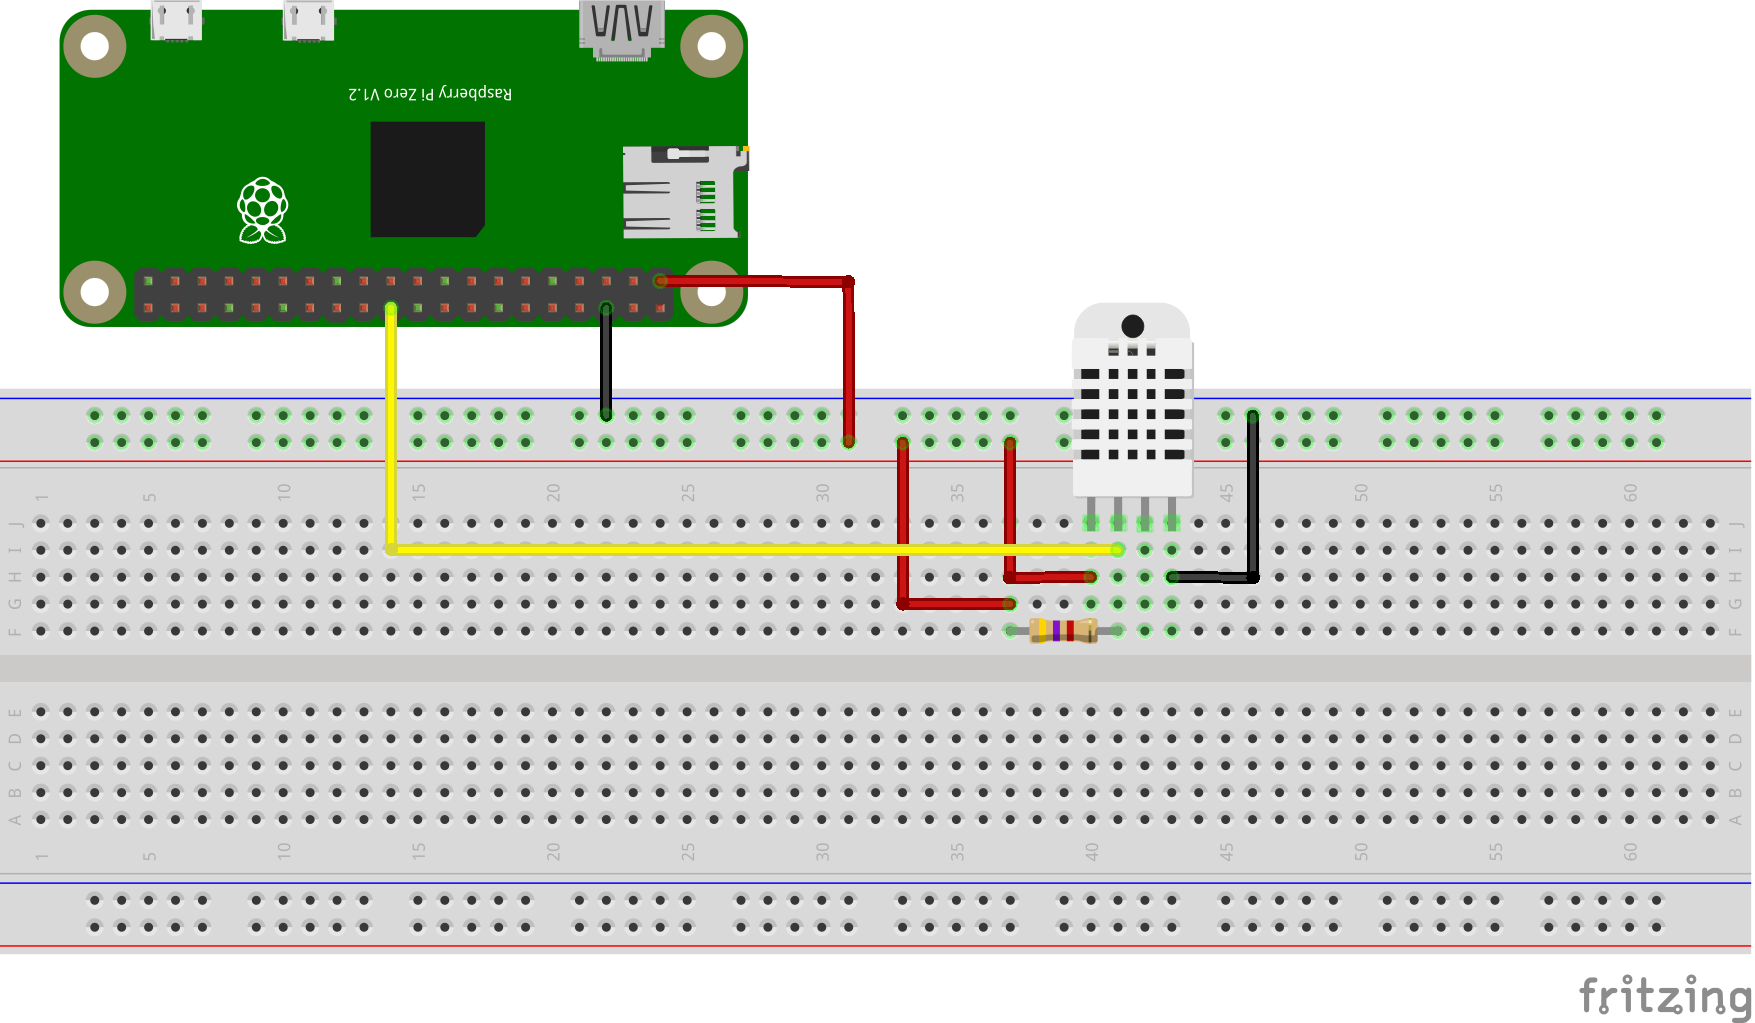
\includegraphics[height=130pt, width=200pt]{sensor}
      \end{center}
    \end{frame}

    \begin{frame}{Funcionamento dos Dispositivos Sensitivos}
      \begin{center}
      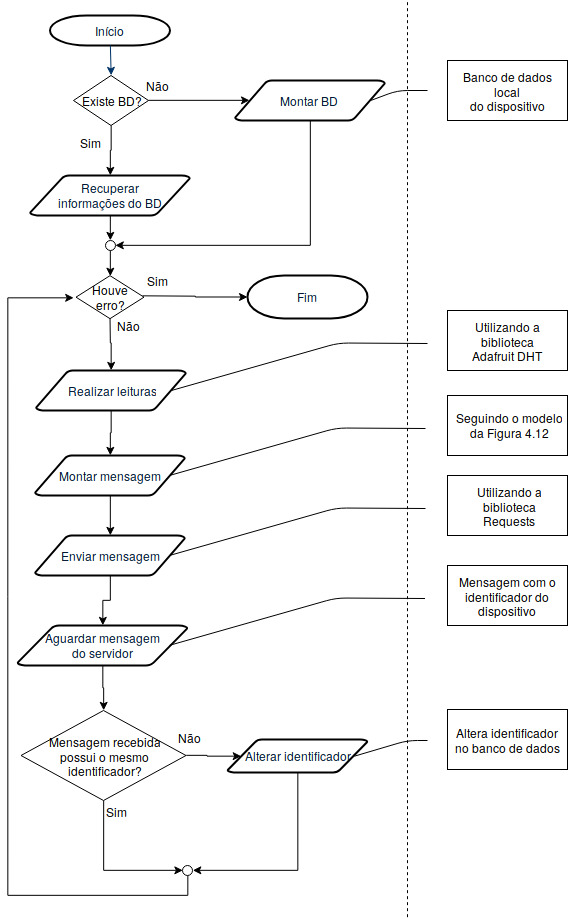
\includegraphics[height=235pt, width=200pt]{fluxogramaSensor}
      \end{center}
    \end{frame}


    \begin{frame}{Interação Sensor-Servidor}
      A interação tem início com um envio, por parte do dispositivo sensitivo, de uma mensagem JSON para o sistema.
      \begin{center}
      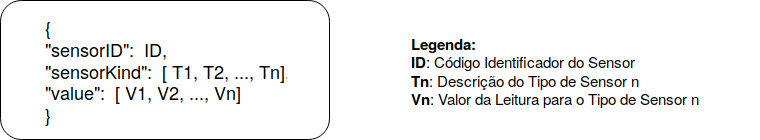
\includegraphics[height=75pt, width=250pt]{mensagemJSON}
      \end{center}
    \end{frame}
    \begin{frame}{Interação Sensor-Servidor}
      A partir do recebimento da mensagem:
      \begin{itemize}
        \item Verifica se o sensor já está cadastrado no sistema;
          \begin{itemize}
            \item Se estiver:
            \begin{itemize}
              \item Armazena as leituras recebidas
            \end{itemize}
            \item Se não estiver:
            \begin{itemize}
              \item Cria um objeto Sensor;
              \item Cria as novas categorias de sensor, caso não existam;
              \item Armazena as leituras recebidas;
              \item Envia o novo código identificador para o dispositivo.
            \end{itemize}
          \end{itemize}
      \end{itemize}
    \end{frame}

    \begin{frame}{Colaboração com o sistema}
      A colaboração basea-se na intenção do usuário em responder as perguntas propostas.
      \begin{center}
      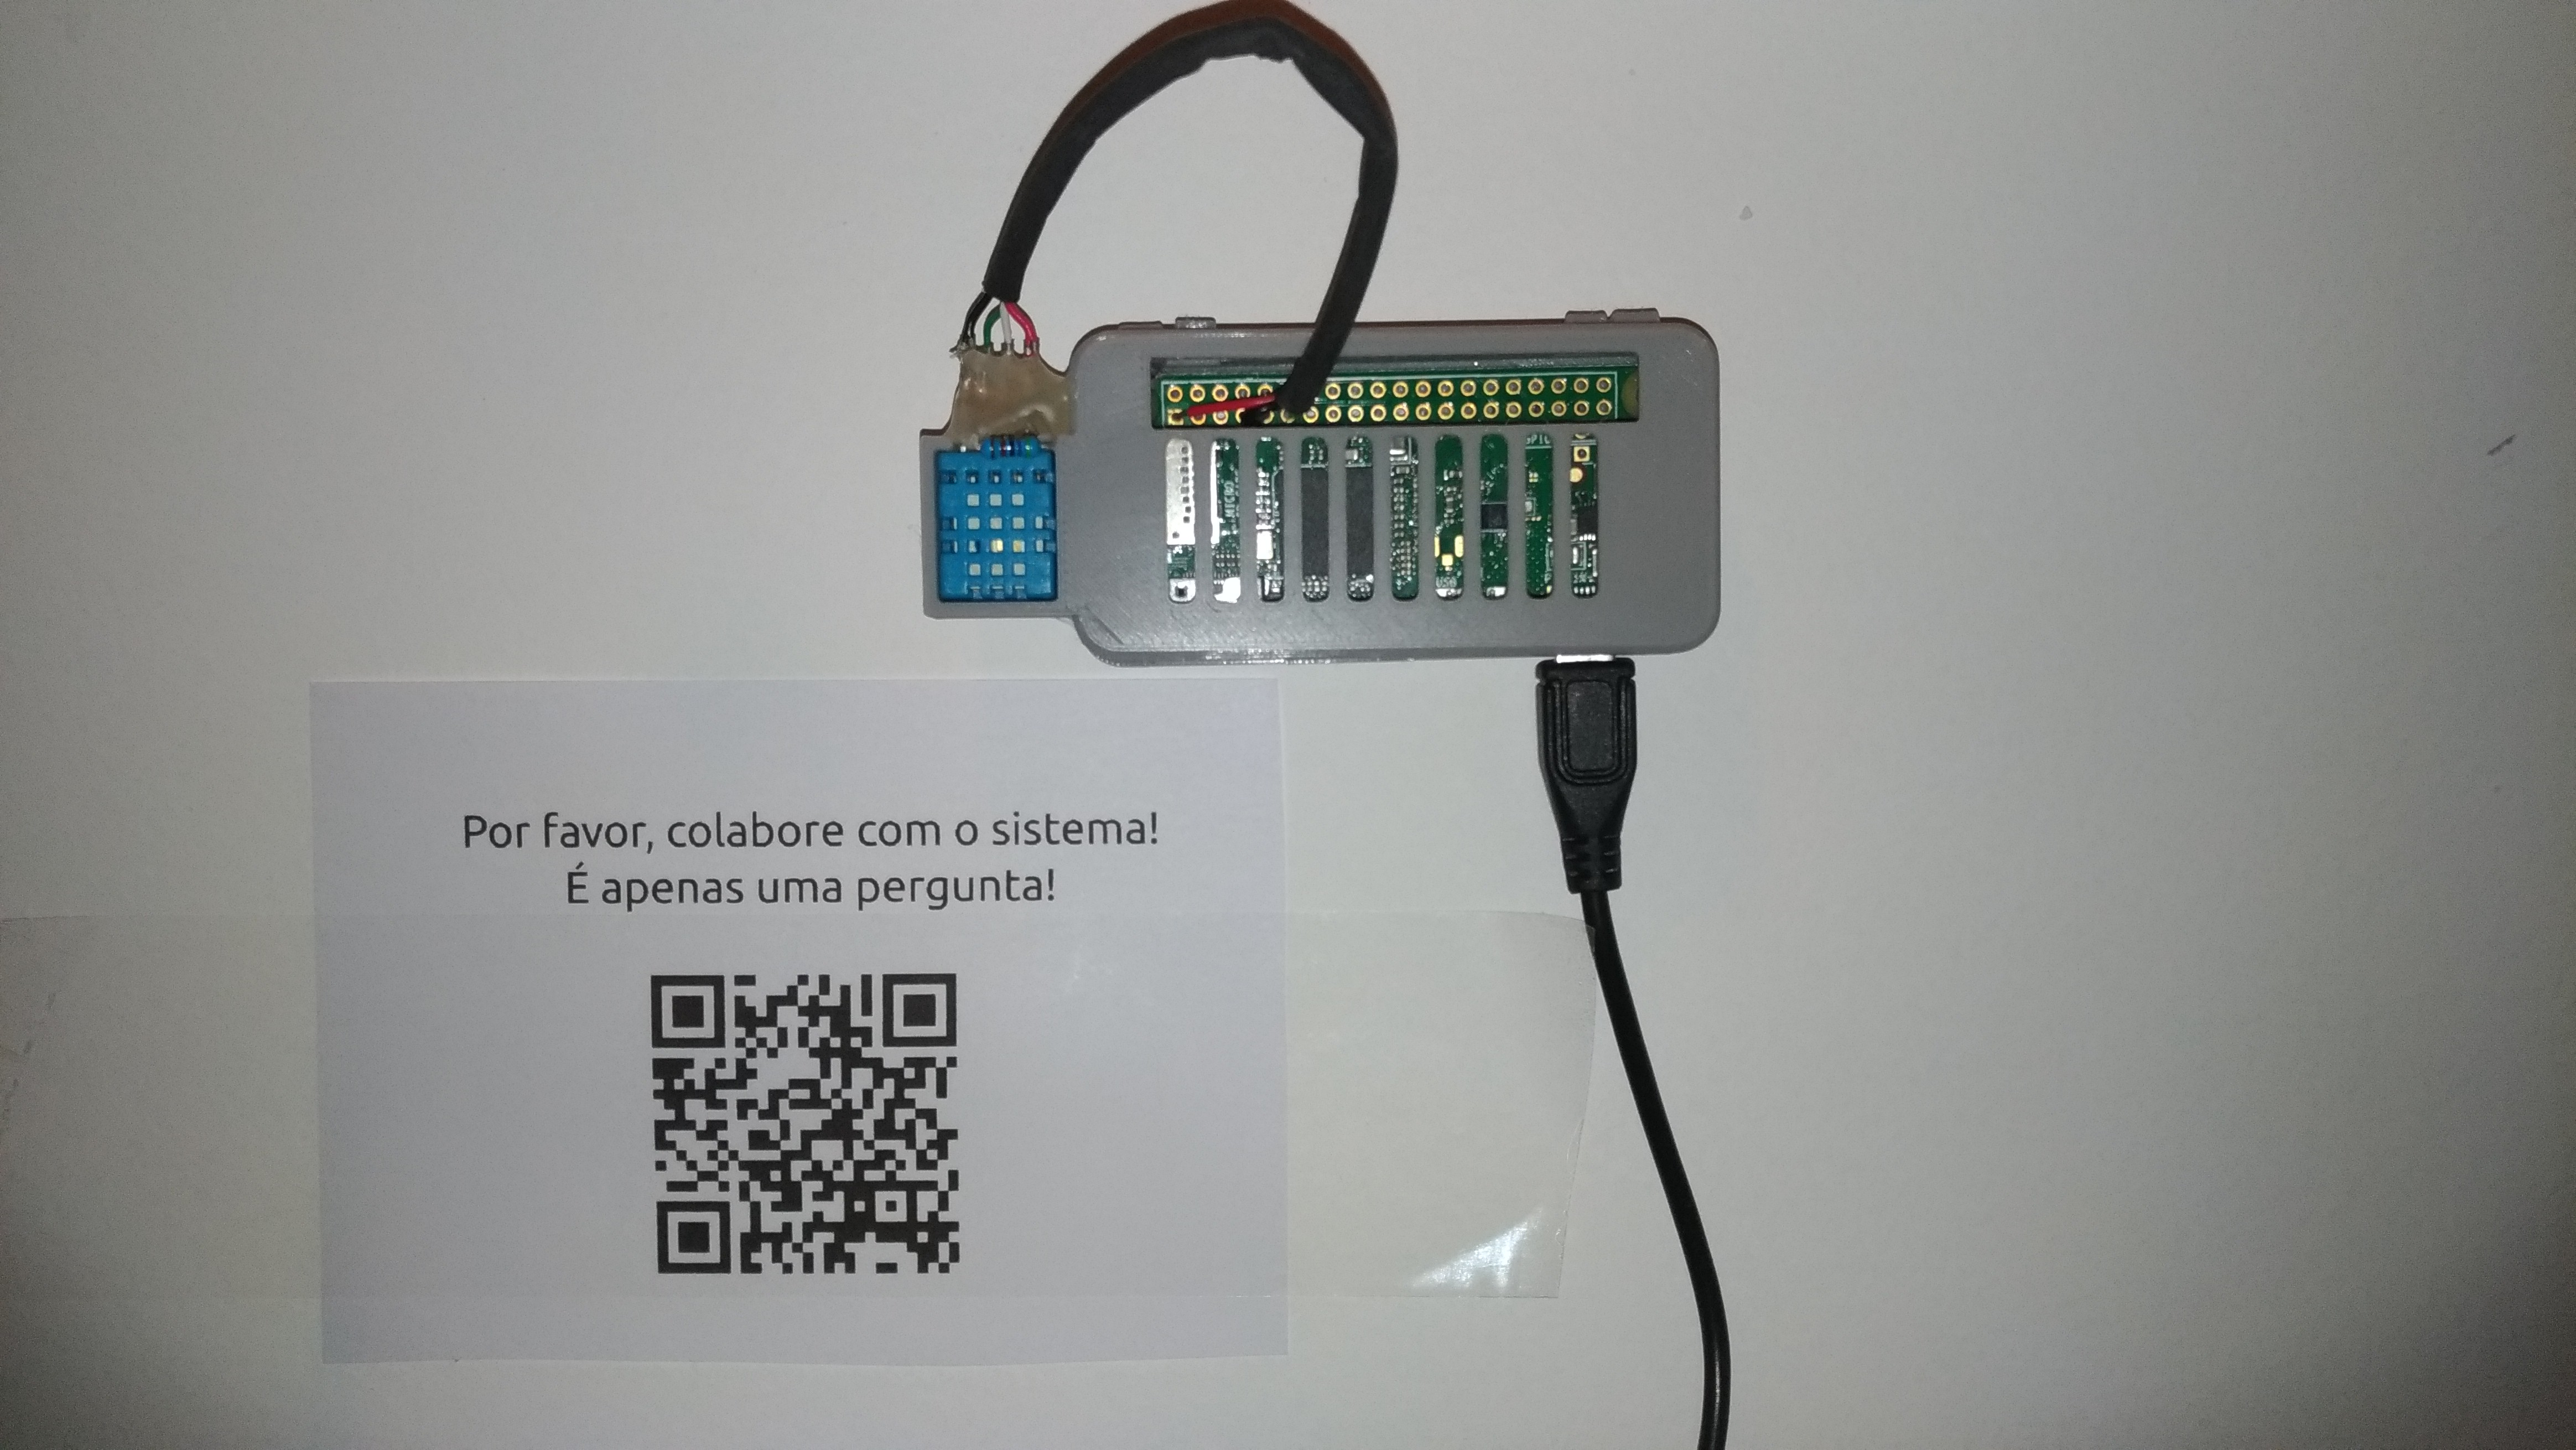
\includegraphics[height=130pt, width=200pt]{sensormsg}
      \end{center}
    \end{frame}

  \section{Resultados}

    \begin{frame}{ Prova de Conceito - Adição de Dispositivos}
      Supondo a construção e configuração de um novo dispositivo, deseja-se verficar se o sistema é capaz de incluí-lo de forma simples e eficaz.
      \begin{center}
      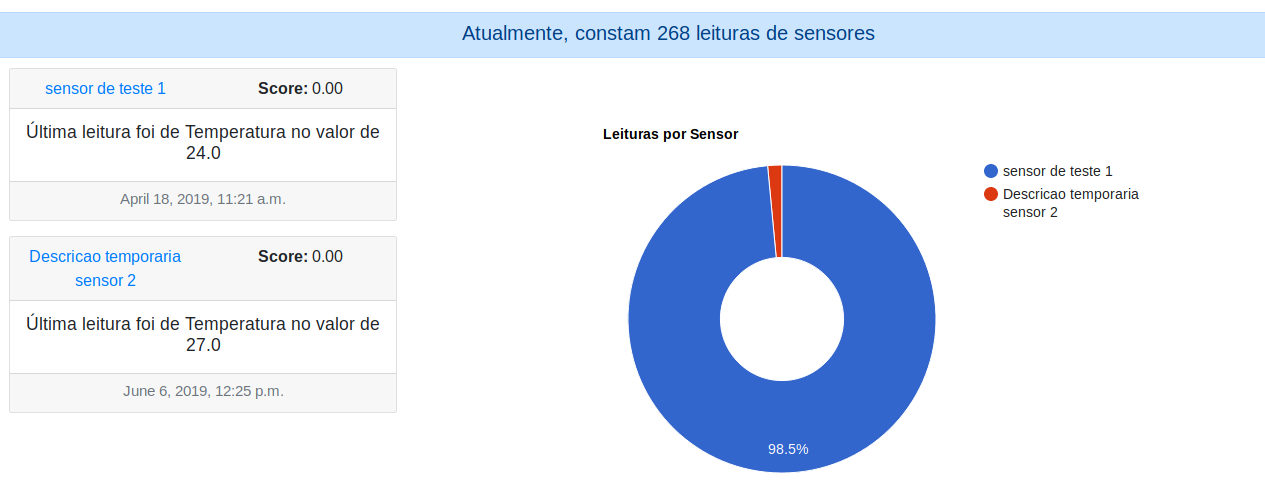
\includegraphics[height=130pt, width=\textwidth]{prova2}
      \end{center}
    \end{frame}
    \begin{frame}{Prova de Conceito - Inspeção dos Dados Coletados}
      É realizada a verificação do armazenamento das leituras enviadas por um dos sensores.
      \begin{center}
      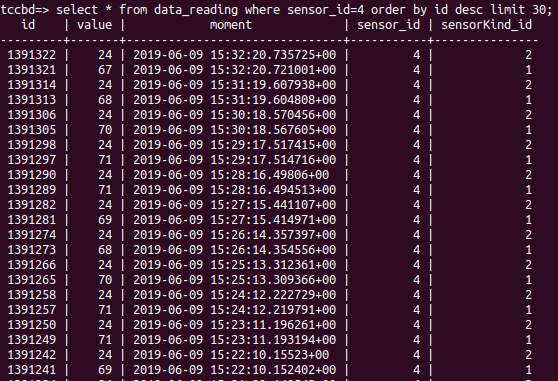
\includegraphics[height=150pt, width=200pt]{prova4}
      \end{center}
    \end{frame}
    \begin{frame}{Prova de Conceito - Simulação de Colaboração por um Usuário}
      Supondo que um usuário se depara com um dos QR-codes localizado próximo a um dos sensores
      \begin{center}
      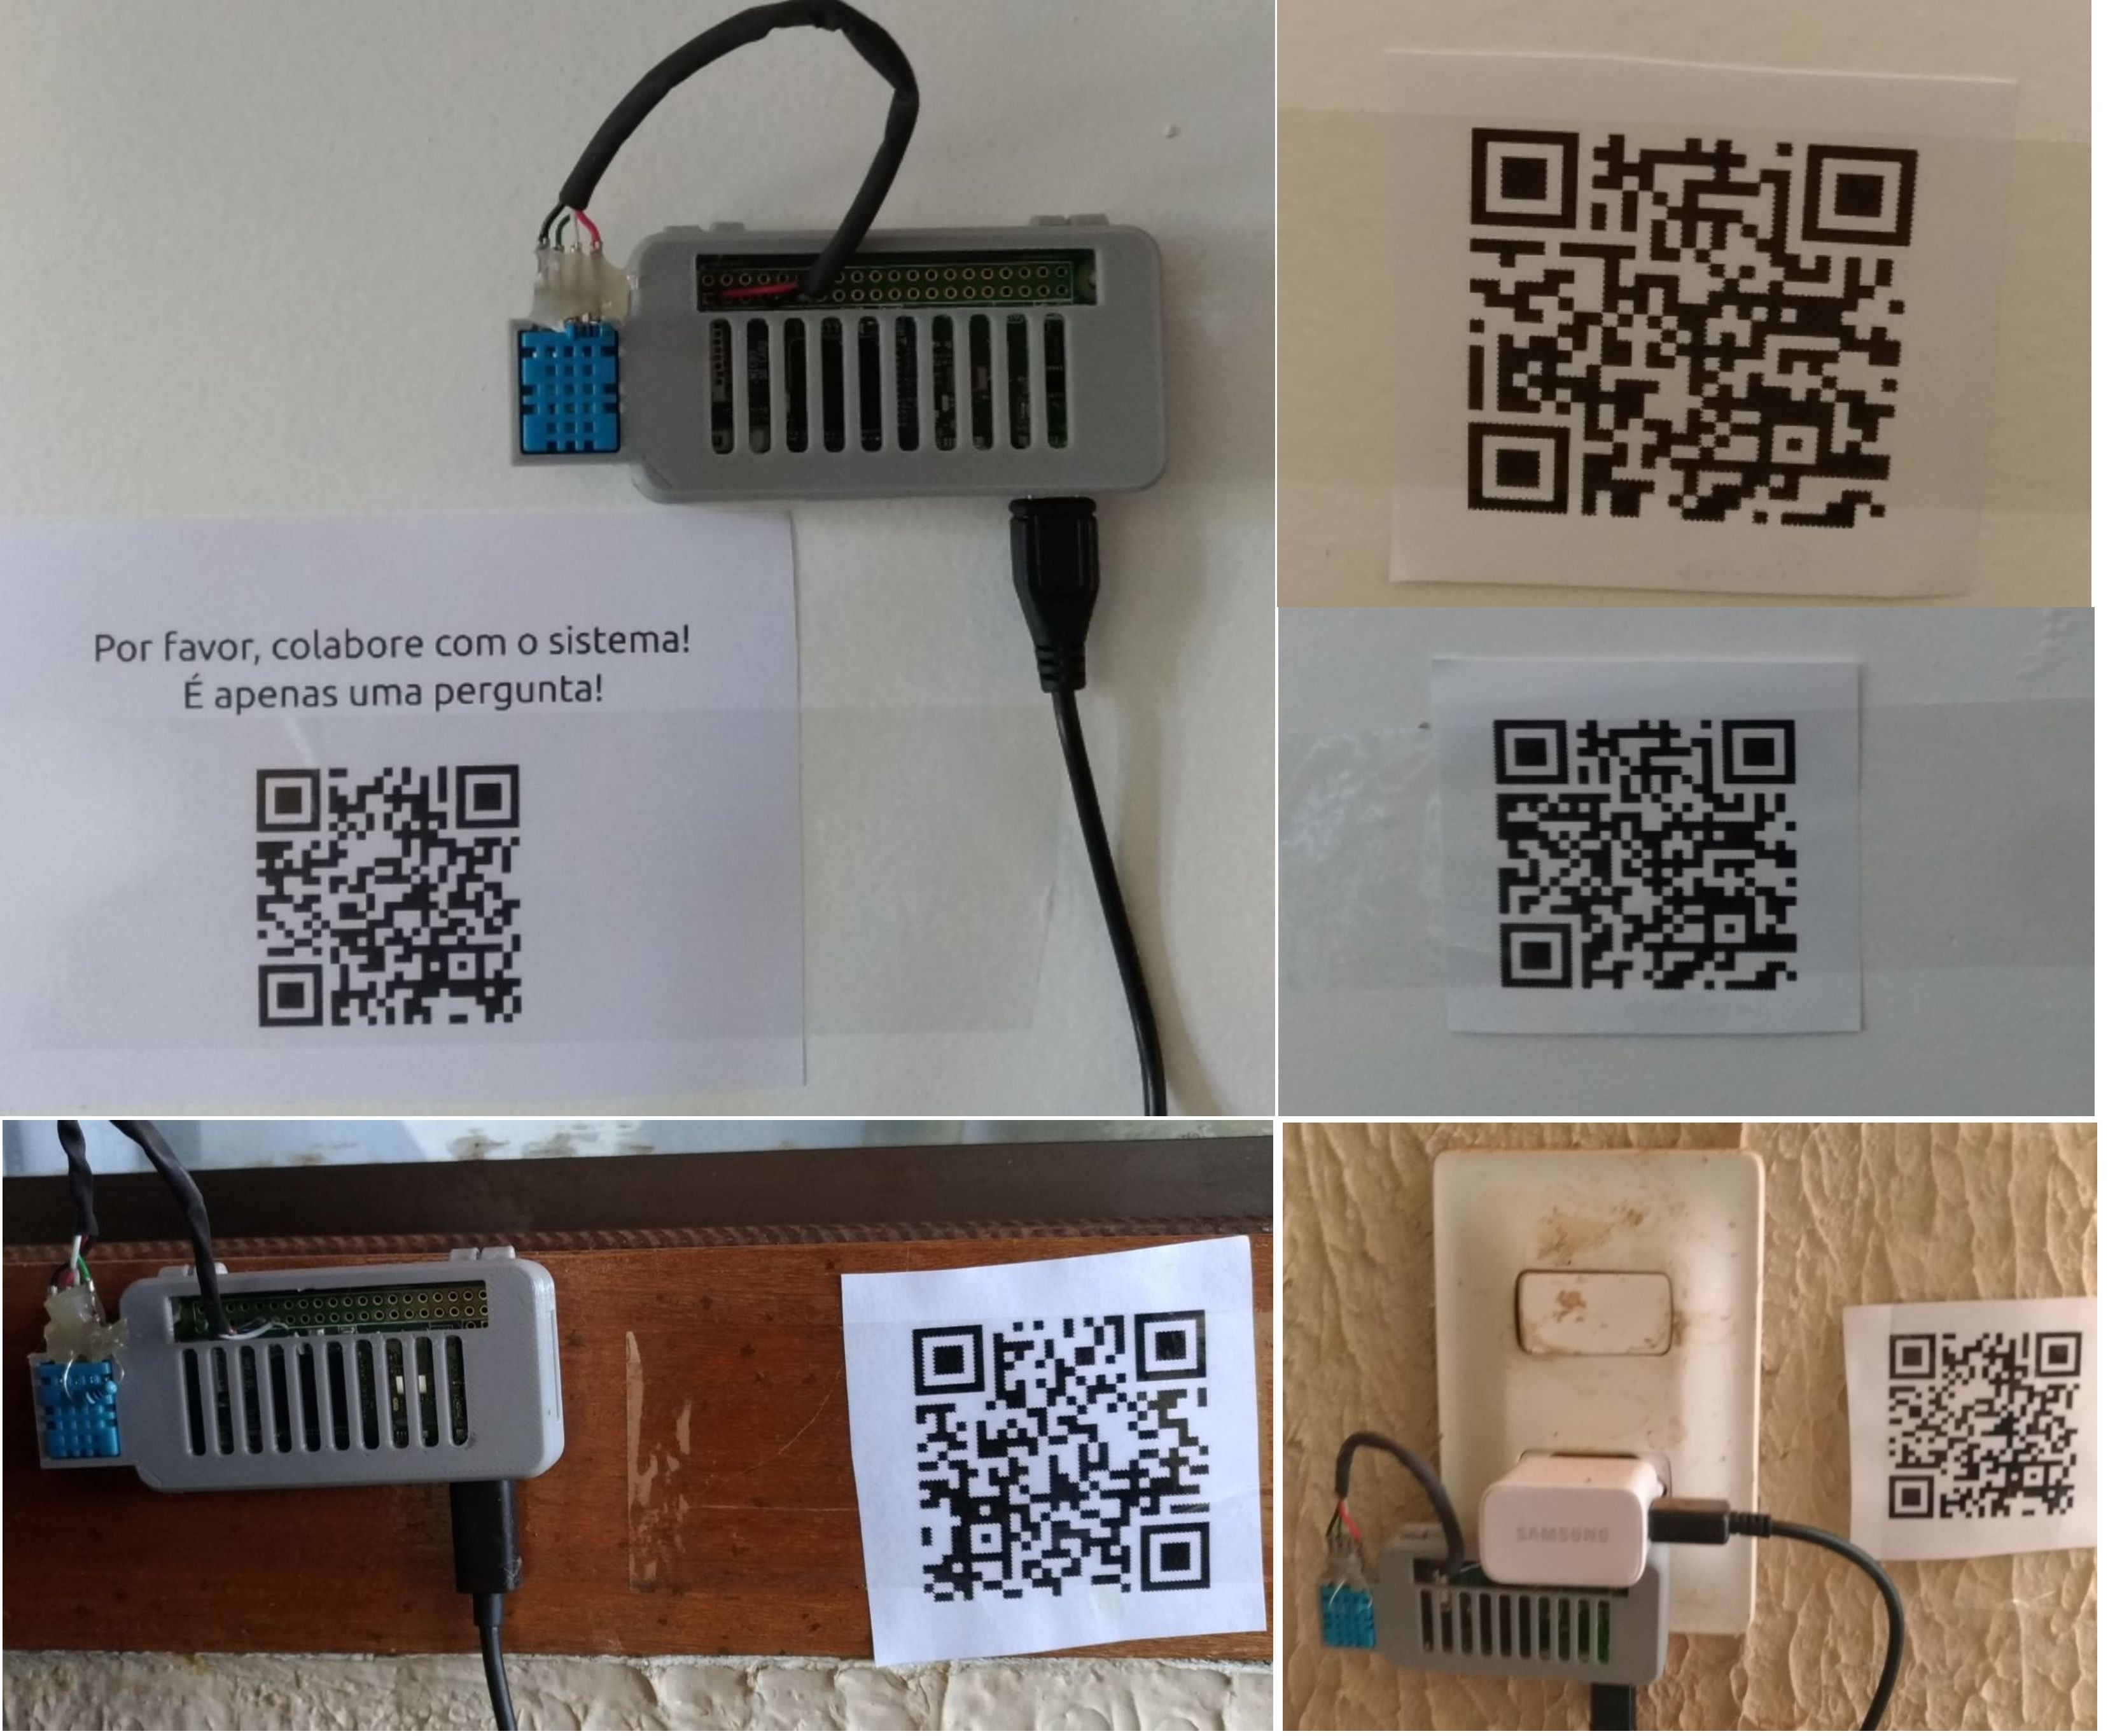
\includegraphics[height=150pt, width=200pt]{prova5}
      \end{center}
    \end{frame}
    \begin{frame}{Prova de Conceito - Simulação de Colaboração por um Usuário}
      \begin{center}
      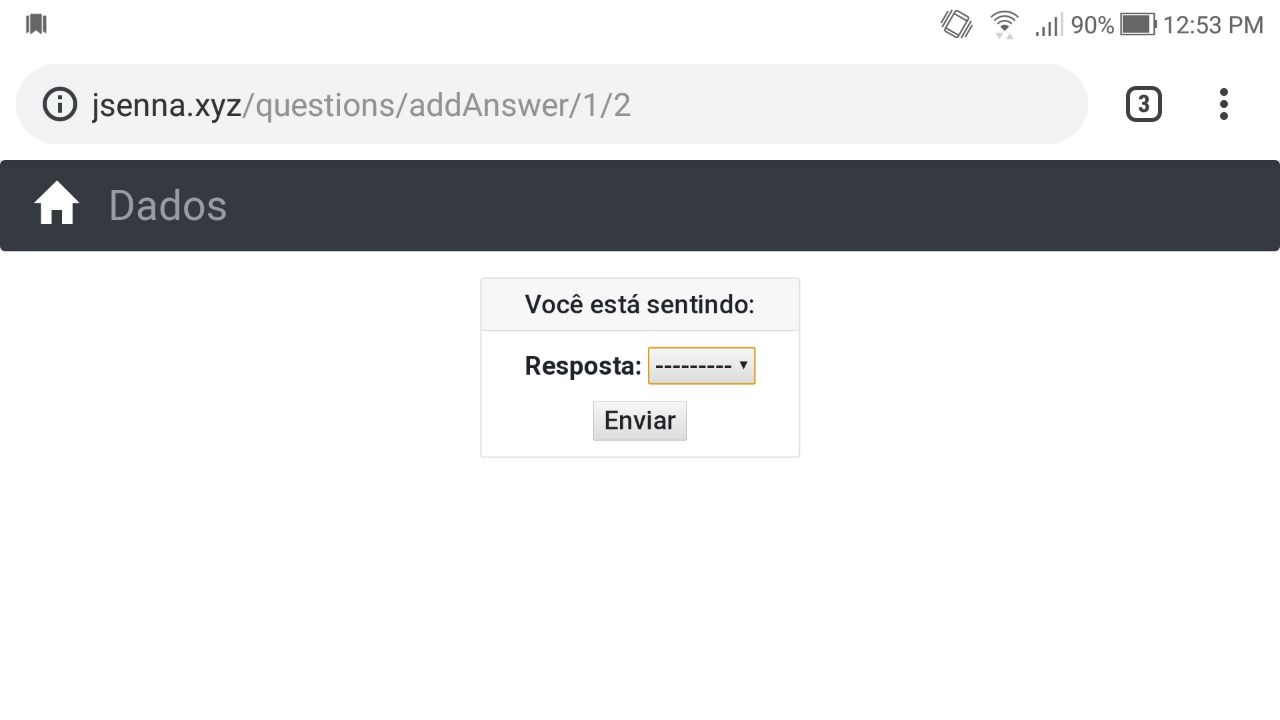
\includegraphics[height=110pt, width=200pt]{prova6}
      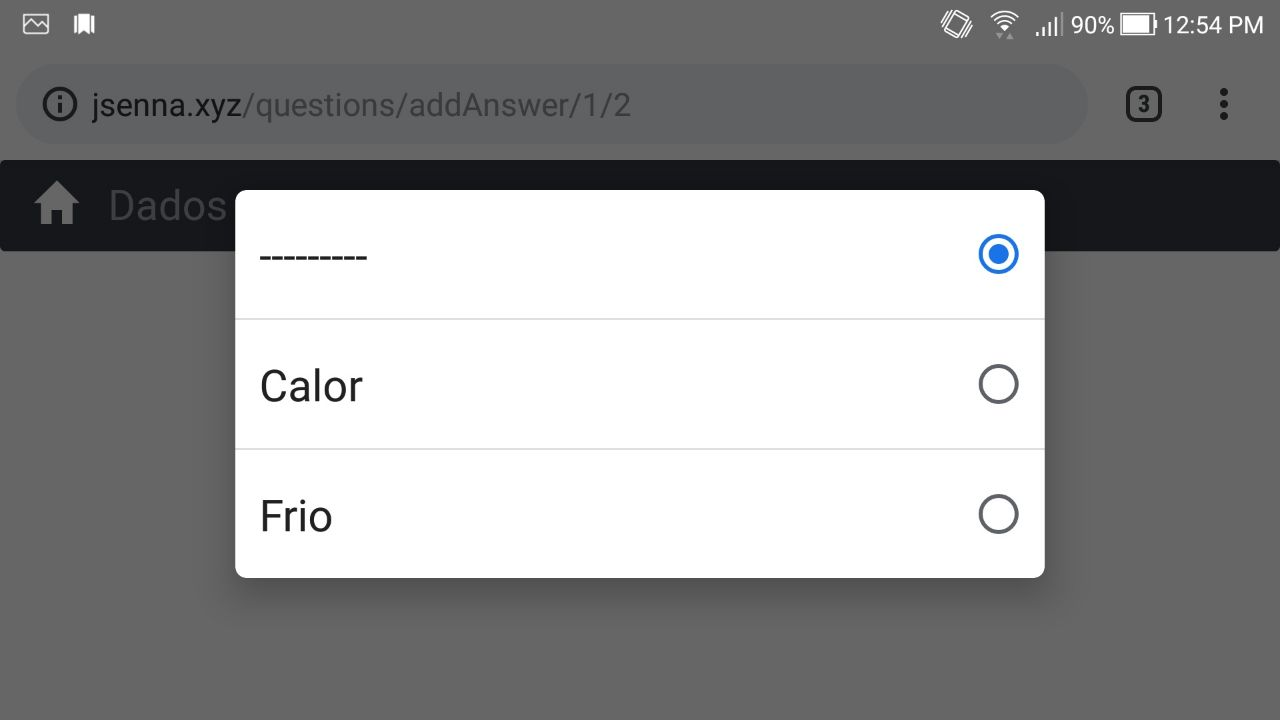
\includegraphics[height=110pt, width=200pt]{prova7}
      \end{center}
    \end{frame}
    \begin{frame}{Prova de Conceito - Simulação de Colaboração por um Usuário}
      \begin{center}
        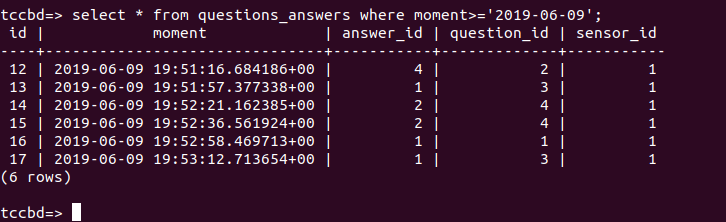
\includegraphics[height=130pt, width=200pt]{prova12}
      \end{center}
    \end{frame}
    \begin{frame}{Prova de Conceito - Utilização do Sistema}
      Supondo um usuário interessado em acessar as informações contidas no sistema
      \begin{center}
      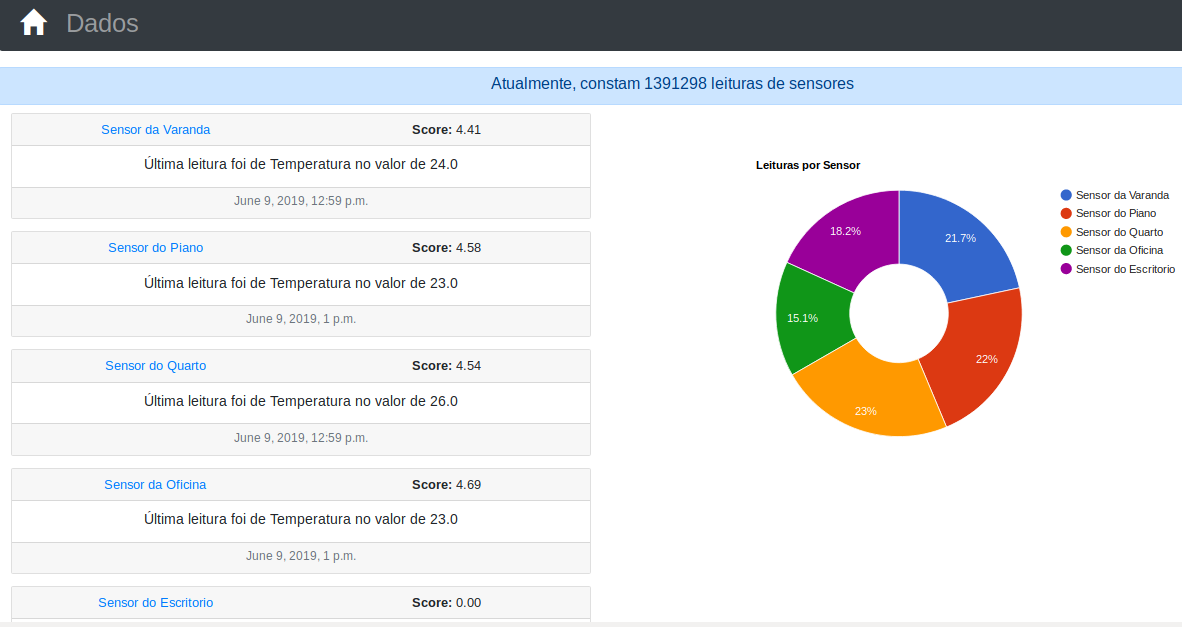
\includegraphics[height=130pt, width=\textwidth]{prova8}
      \end{center}
    \end{frame}
    \begin{frame}{Prova de Conceito - Utilização do Sistema}
      \begin{center}
        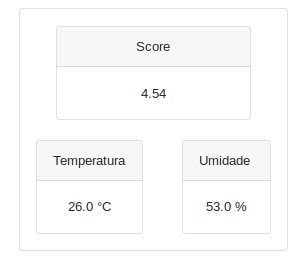
\includegraphics[height=90pt, width=140pt]{prova9}
        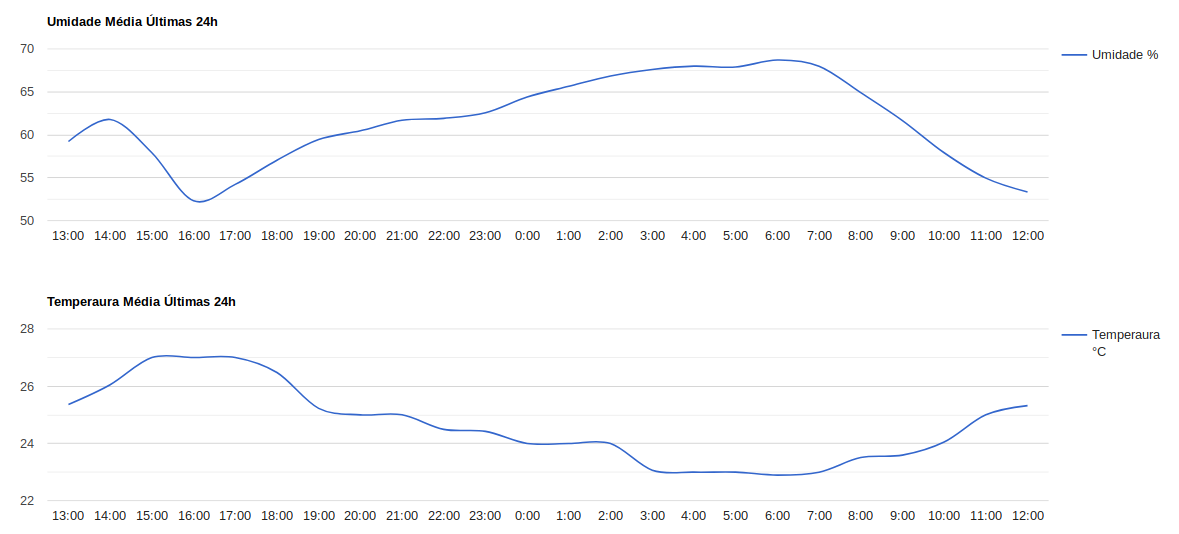
\includegraphics[height=130pt, width=\textwidth]{prova10}
      \end{center}
    \end{frame}
    \begin{frame}{Prova de Conceito - Utilização do Sistema}
      \begin{center}
        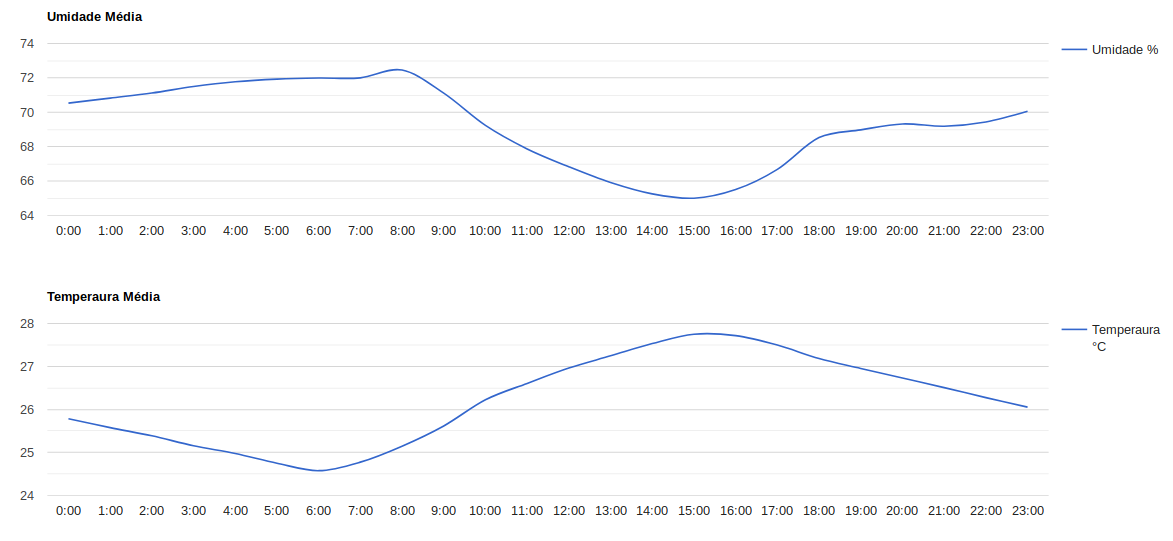
\includegraphics[height=130pt, width=\textwidth]{prova11}
      \end{center}
    \end{frame}
    \begin{frame}{Teste Comparativo - Visão Geral}
      \null \quad O período considerado foi do dia 12/02/2019 ao dia 17/05/2019 (95 dias). Durante esse intervalo foram coletados 1.091.516 leituras.
      \\\null \quad Para a comparação com a métrica implementada pelo sistema, foi utilizada a \textit{Overall Equipment Effectiveness} (OEE) \cite{artigoOEE}. %, uma métrica quantitativa utilizada na indústria para medir diferentes tipos de perda de eficiência de um equipamento e indicar áreas para aperfeiçoamento do processo de produção \cite{artigoOEE}.
      \\\null \quad Para o cálculo da OEE, é preciso calcular três elementos: Disponibilidade, Produtividade e Qualidade.
    \end{frame}
    \begin{frame}{Teste Comparativo - OEE - Disponibilidade}
      A disponibilidade é a razão entre o tempo de funcionamento útil e o tempo de funcionamento total.
      Considera-se um dia útil o dia em que foram armazenadas mais do que a metade do total de leituras esperadas por dia
      \begin{center}
      % \captionof{table}{Tabela que representa a disponibilidade dos sensores.}\label{disponibilidade}
      \resizebox{\textwidth}{!}{%
      \begin{tabular}{rrrrr}
        \hline
        Sensor     & \begin{tabular}[c]{@{}l@{}}Número de dias\\  em funcionamento (N)\end{tabular} & \begin{tabular}[c]{@{}l@{}}Tempo útil\\em dias (U)\end{tabular} & \begin{tabular}[c]{@{}l@{}}Tempo de\\  não funcionamento\\em dias (I)\end{tabular} & Disponibilidade (D) \\
      \hline
      Oficina    & 53                                                                             & 49                 & 4                                                                     & 92,45\%             \\
      \hline
      Escritório & 95                                                                            & 89                 & 6                                                                     & 93,68\%             \\
      \hline
      Quarto     & 95                                                                            & 93                 & 2                                                                     & 97,89\%             \\
      \hline
      Varanda    & 95                                                                            & 87                 & 8                                                                     & 91,57\%             \\
      \hline
      Piano      & 95                                                                            & 89                 & 6                                                                     & 93,68\%

      \end{tabular}%
      }
      \end{center}
    \end{frame}
    \begin{frame}{Teste Comparativo - OEE - Produtividade}
      A Produtividade de um equipamento é dada pela razão entre a quantidade produzida e a quantidade esperada
      \begin{center}
      \resizebox{\textwidth}{!}{%
      \begin{tabular}{lrrrr}
        \hline
      Sensor     & \multicolumn{1}{l}{\begin{tabular}[c]{@{}l@{}}Número de dias\\  em funcionamento (N)\end{tabular}} & \multicolumn{1}{l}{Número de leituras (L)} & \multicolumn{1}{l}{\begin{tabular}[c]{@{}l@{}}Número de leituras\\  esperado (E)\end{tabular}} & \multicolumn{1}{l}{Disponibilidade (D)} \\
      \hline
      Oficina    & 53                                                                                                 & 140754                                     & 152640                                                                                         & 92,21\%                                 \\
      \hline
      Escritório & 95                                                                                                 & 233500                                     & 273600                                                                                         & 85,34\%                                 \\
      \hline
      Quarto     & 95                                                                                                 & 246550                                     & 273600                                                                                         & 90,11\%                                 \\
      \hline
      Varanda    & 95                                                                                                 & 233722                                     & 273600                                                                                         & 85,42\%                                 \\
      \hline
      Piano      & 95                                                                                                 & 236990                                     & 273600                                                                                         & 86,62\%
      \end{tabular}%
      }
      \end{center}
    \end{frame}
    \begin{frame}{Teste Comparativo - OEE - Qualidade}
      Neste trabalho não foi verificada a qualidade do dado produzido. Entretanto para que fosse possível calcular a OEE, a Qualidade foi considerada 100\%.
    \end{frame}
    \begin{frame}{Teste Comparativo - OEE}
        Multiplicando os três elementos, obtêm-se a OEE.
        \begin{center}

        \resizebox{\textwidth}{!}{%
        \begin{tabular}{lrrrr}
          \hline
        Sensor     & \begin{tabular}[c]{@{}l@{}}Disponibilidade (D)\end{tabular} & Produtividade (P) & \begin{tabular}[c]{@{}l@{}}Qualidade (Q)\end{tabular} & OEE \\
        \hline
        Oficina    & 92,45\%                                                                             & 92,21\%                 & 100\%                                                                     & 85,24\%             \\
        \hline
        Escritório & 93,68\%                                                                            & 85,34\%                 & 100\%                                                                     & 79,94\%             \\
        \hline
        Quarto     & 97,89\%                                                                            & 90,11\%                 & 100\%                                                                     & 88,20\%             \\
        \hline
        Varanda    & 91,57\%                                                                            & 85,42\%                & 100\%                                                                     & 78,22\%             \\
        \hline
        Piano      & 93,68\%                                                                            & 86,62\%                & 100\%                                                                     & 81,15\%
        \end{tabular}%
        }
        \end{center}
    \end{frame}
    \begin{frame}{Teste Comparativo - OEE vs SenseHera}
      Comparação entre OEE e SenseHera:
      \begin{center}
      \resizebox{170}{!}{%
      \begin{tabular}{lrr}
        \hline
      Sensor     & \multicolumn{1}{l}{OEE} & \multicolumn{1}{l}{\begin{tabular}[c]{@{}l@{}}Pontuação\\ Calculada\end{tabular}} \\
      \hline
      Oficina    & 85,24\%                 & 88\%                                                                              \\
      \hline
      Escritório & 79,94\%                 & 84,4\%                                                                            \\
      \hline
      Quarto     & 88,20\%                 & 89\%                                                                              \\
      \hline
      Varanda    & 78,22\%                 & 83,6\%                                                                            \\
      \hline
      Piano      & 81,15\%                 & 85,7\%

      \end{tabular}%
      }
      \end{center}
    \end{frame}
  \section{Conclusão}
    \begin{frame}{ Conclusão }
      Este trabalho apresentou:
      \begin{itemize}
        \item O desenvolvimento de sistema SenseHera;
        \item A construção de um ambiente IoT em escala reduzida;
        \item O teste comparativo entre o sistema implementado e uma métrica utilizada na indústria.
      \end{itemize}
    \end{frame}

    \begin{frame}{Trabalhos Futuros}
      Os temas a seguir tratam sobre trabalhos futuros:
      \begin{itemize}
        \item Implementação do sistema utilizando bancos de dados NOSQL;
        \item Associar as informações fornecidas pelos usuários aos registros dos sensores por meio de metadados;
        \item Implementação de uma ontologia para fornecer semântica aos dados;
        \item Permitir o envio de informações mais complexas aos sensores.
      \end{itemize}

    \end{frame}

  \begin{frame}{Referências}
    \setbeamertemplate{bibliography item}[text]
    \bibliography{bibliografia}
    \bibliographystyle{ieeetr}
  \end{frame}


  \begin{frame}
    \begin{center}
      Obrigado!
      \begin{center}
        \includegraphics[scale=0.05]{hera}
      \end{center}
    \end{center}
  \end{frame}
\end{document}
